\documentclass[a4paper,10pt]{scrartcl}
\usepackage{fancyhdr}
\usepackage[utf8]{inputenc}
\usepackage[ngerman]{babel}
\usepackage{enumerate}
\usepackage[top=2cm, left=2cm, bottom=2cm, right=2cm]{geometry}
\usepackage{graphicx}
\usepackage{listings}
\usepackage{amsmath}
\usepackage{amsfonts}
\usepackage{amssymb}
\usepackage{float}


\pagestyle{fancy}
\headheight30pt
\fancyhf{}
\fancyhead[L]{\begin{small}Computer Graphics 2\\Übungsblatt 4\\Gruppe 5\end{small}}
\fancyhead[R]{\begin{small}Stürmer, Felix - 230127 - Informatik(Diplom) - stuermer@cs.tu-berlin.de\\
  Oskamp, Robert - 306952 - Mathematik(Diplom) - robert.oskamp@gmx.de\\
  Olthoff, Inken - 305844 - Mathematik(Diplom) - some-body@gmx.de\\
  Neumann, Cedrik - 301635 - Mathematik(Diplom) - c.neumann@live.de\end{small}}
\renewcommand{\headrulewidth}{0.4pt}


\begin{document}
\vspace*{5pt}
\begin{enumerate}[1.]

\item Es gilt
 \begin{itemize}
  \item Die implizite Fläche hat ein Inneres und ein Äußeres, ist also geschlossen. Damit ist das durch Tesselierung entstehende Dreiecksnetz auch geschlossen.
  \item Die implizite Fläche ist zusammenhängend. Damit ist das durch Tesselierung entstehende Dreiecksnetz auch zusammenhängend.
  \item Gäbe es zwei zu einem Punkt p inzidente Polygone $Q_1$, $Q_2$, die keine zu p inzidente gemeinsame Kante haben, dann wäre das Innere der impliziten Fläche nicht zusammenhängend. Also müssen $Q_1$ und $Q_2$ eine zu p inzidente gemeinsame Kante haben.
 \end{itemize}
Das durch Tesselierung entstehende Dreiecksnetz ist also ein Polyeder.

\item Das Entfernen einer Kante aus einem Dreiecksnetz darf nicht vorgenommen werden, wenn es sich bei der Kante um eine Randkante des Netzes handelt, da in diesem Fall Informationen über den Umriss des Netzes unwiederherstellbar verloren gehen.

\item
 \begin{enumerate}[a.]
  \item Skizze des Vorgangs:\\
  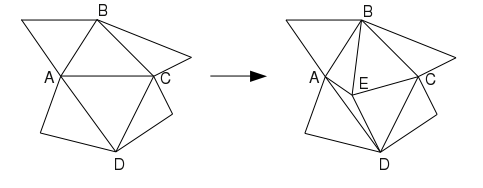
\includegraphics[scale=0.6]{cg2_ex4_3a.png}\\
  Folgende Änderungen müssen am Inhalt der Halbkanten-Datenstruktur vorgenommen werden:
  \begin{itemize}
   \item Füge neuen Knoten E mit seinen Koordinaten und dem entsprechenden Halbkanten Pointer in die Vertexlist ein
   \item Entferne die Halbkanten zu AC aus der Half-Edgelist
   \item Aktualisiere die Faces ABC und ACD zu ABE und AED mit entsprechenden Halbkanten Pointern in der Facelist
   \item Füge neue Halbkanten für AE, BE, CE und DE jeweils mit entsprechenden Startknoten, next, prev und opp Pointern in die Half-Edgelist ein
   \item Füge neue Faces BCE und ECD mit entsprechenden Halbkanten Pointern in die Facelist ein
   \item Aktualisiere in der Half-Edgelist die Pointer next und prev der Halbkanten für AB, BC, CD und DA
  \end{itemize}

  \item Skizze des Vorgangs:\\
  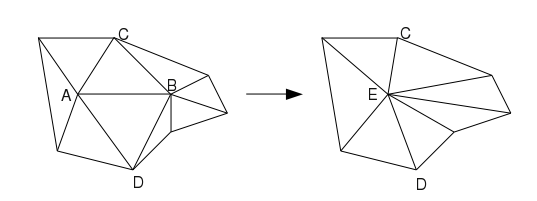
\includegraphics[scale=0.6]{cg2_ex4_3b.png}\\
  Folgende Änderungen müssen am Inhalt der Halbkanten-Datenstruktur vorgenommen werden:
  \begin{itemize}
   \item Entferne Knoten B aus der Vertexlist
   \item Entferne Halbkanten zu AB aus der Half-Edgelist
   \item Entferne die Halbkanten zu den Faces ACB und ABD aus der Half-Edgelist
   \item Entferne Faces ACB und ABD aus der Facelist
   \item Aktualisiere den opp und gegebenenfalls Startknoten Pointer der verbleibenden Halbkanten zu AC, CB, BD und AD in der Half-Edgelist
   \item Füge neuen Knoten E mit seinen Koordinaten und dem entsprechenden Halbkanten Pointer in die Vertexlist ein
   \item Aktualisiere in der Half-Edgelist die next, prev und gegebenenfalls Startknoten Pointer der anderen mit A oder B inzidenten Halbkanten entsprechend
   \item Aktualisiere den Halbkanten Pointer der Knoten C und D in der Vertexlist
  \end{itemize}
 \end{enumerate}

\newpage

\item Zur lokalen Abschätzung der Approximationsqualität eines Dreiecksnetzes in Bezug auf eine implizite Fläche betrachte die Kantenmenge $E$ derjenigen Kanten des Dreiecksnetzes, die in dem betrachteten lokalen Gebiet liegen. Für einen Knoten $v$ sei der Abstand $d(v)$ zu der impliziten Fläche gegeben durch den Abstand des zu $v$ gehörigen Punktes zur impliziten Fläche entlang der Flächennormale. Für jede Kante $e \in E$ mit Endknoten $v_1$ und $v_2$ berechne den Abstand zur impliziten Fläche wie folgt: $d(e) = d(v_1) + d(v_2)$. Die Funktion, die lokal die Approximationsqualität schätz, sei dann gegeben durch $d(E) = max\{d(e) | e \in E\}$.

\item Aus einem Sechseckgitter, wie wir es hier haben
\begin{center}
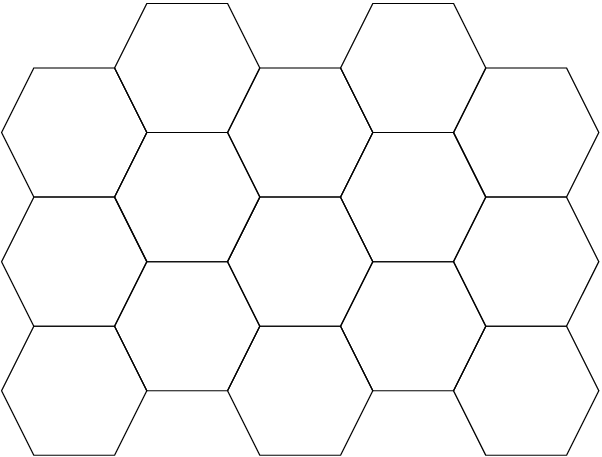
\includegraphics[scale=0.25]{cg2_ex4_4-1.png}\\
\end{center}
kann man durch einf\"ugen von Hilfsknoten (rot) aus jedem der Sechsecke sechs Dreiecke machen und erh\"alt dadurch ein Dreiecksgitter.
\begin{center}
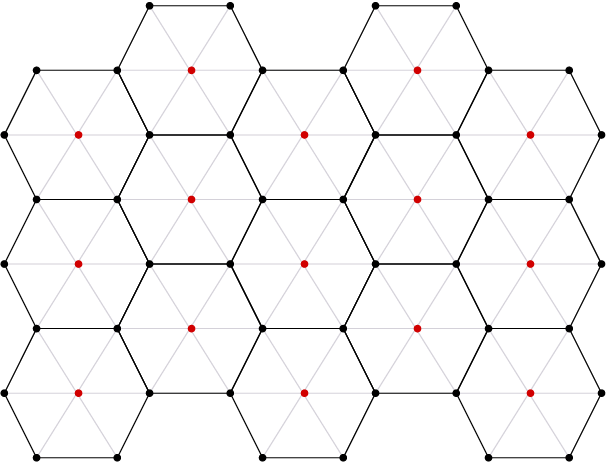
\includegraphics[scale=0.25]{cg2_ex4_4-2.png}\\
\end{center}
Dieses Dreiecksgitter k\"onnen wir nun wie in der Vorlesung besprochen verfeinern, wobei wir sp\"ater nur Verfeinerungsknoten verwenden wollen, die auf den Hilfskanten liegen. (Das hei\ss t rote Knoten sind nur zur Hilfe da und werden sp\"ater nicht mehr gebraucht.)
\begin{center}
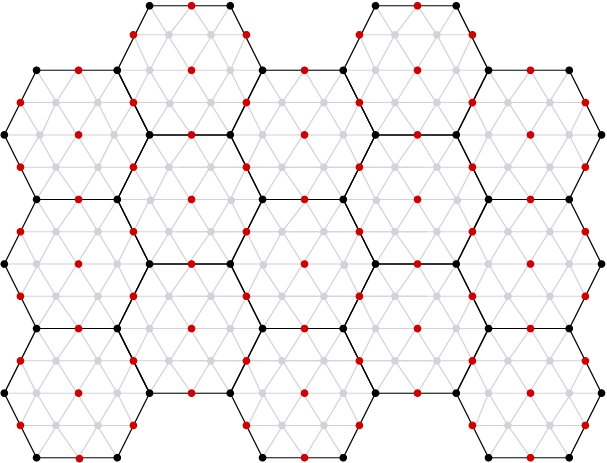
\includegraphics[scale=0.25]{cg2_ex4_4-3.png}\\
\end{center}
Aus dem verfeinerten Dreiecksgitter k\"onnen wir dann wieder ein Sechseckgitter erhalten, indem wir jeweils die sechs Dreiecke um einen roten Hilfsknoten herum zu einem Sechseck zusammenf\"ugen.
\begin{center}
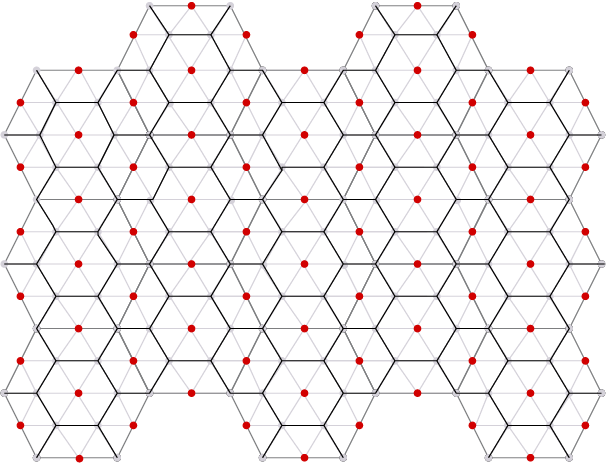
\includegraphics[scale=0.25]{cg2_ex4_4-4.png}\\
\end{center}

\end{enumerate}
\end{document}
